Le domaine de compression des graphes est assez récent, toutefois, il a conne une grande évolution vue son importance. Une multitudes de méthodes ont été proposées au cours des années, ces méthodes différent l'une de l'autre sur plusieurs points comme : le type de graphe en entrée, le type de structure en sortie, type de la compression et les technique utilisés pour la compression. En ce basant sur cette différence, plusieurs classification ont été suggérés. Nous allons dans ce qui suit présenter les plus importantes parmi ces classifications.\\

Dans \citep{maneth2015survey}, les auteurs proposent une classification basée au début sur le type de compression, ils regroupent les méthodes en deux catégories principales : méthodes de compression sans perte et méthode de compression avec perte. Les méthodes de compression sans perte sont divisés à leurs tours  en trois classes selon le type de structures récupérés en sortie. La première classe est la représentation succinct, les méthodes de cette classe représentent le graphe sous forme d'une chaine de bits succincte irréversible lors de la décompression, la sortie de ces méthodes est une structure compacte du graphe original. Parmi les méthode de cette classe, nous trouvons : Web Framework de Boldi et Vigna \citep{boldi2004webgraph}. La deuxième classe est la représentation structurelle. Contrairement à l'approche précédente, les méthodes de cette classe modifient en quelques sorte la structure du graphe initial, sachant que les modifications apportés sont réversibles. La sortie sera donc une structure réduite et non pas compacte de la version initial. Entre ces méthodes, nous citons : RePair de Claude et Navarro \citep{claude2010fas}. La dernière catégorie est la compression RDF qui est assez récente, les méthodes de cette classe sont appliqués sur les bases de donnés RDF, nous trouvons parmi ces techniques : Dcomp de \citep{martinez2012compression} . Les méthodes de compression avec perte quand a eux apportent des modifications irréversible sur le graphe en supprimant les informations redondantes et le bruit. Comme exemple, nous citons : ASSG de \citep{zhang2014assg}.\\

Une autre classification a été exposé par Lui et al. dans \citep{liu2018graph} qui classe les méthodes sur trois niveaux. Au premier et deuxième niveaux, les techniques de compression sont regroupés en fonction du type de graphe en entrée selon deux critères : graphe statique où dynamique et graphe simple où étiqueté. Pour le troisième niveau, les auteurs catégorisent les méthodes selon la technique de traitement utilisé. Quatre catégories sont définies: les méthodes de regroupement où agrégation, ces méthodes permettent d'agréger de manière récursive un ensemble de nœuds où liens où carrément un cluster en un super nœud où un nœud virtuel, comme exemple de ces techniques, nous trouvons Grass \citep{lefevre2010grass}. Le deuxième type de méthodes sont les méthodes de compression de bits, ces méthodes minimisent le nombre de bits nécessaire au stockage du graphe en se basant sur le principe de description minimal MDL, elles peuvent être sans où avec perte, parmi eux, nous citons LSH-based \citep{khan2014set}. la troisième classe est les méthodes de simplification qui suppriment les arrêtes inutiles et inintéressantes, entres ces méthodes, nous trouvons \citep{shen2006visual}. La dernière catégorie est l'influence, les méthodes de cette catégorie décrivent le graphe par les flux d'influence les plus importantes ce qui permet de l'analyser plus facilement, ces méthodes permettent de formuler le problème de compression comme un processus d'optimisation dans lequel la quantité de donnés liée à l'influence est maintenue en sortie, parmi ces technique, nous motionnons \citep{shi2015vegas}.\\


La dernière classification que nous allons voir est la classification proposé dans le master de l'année passée par Belhocine et Guermah \citep{master2017}. Cette classification s'appuie sur les taxonomies des différents techniques de compression existantes dans la littérature en se basant sur les classifications précédentes. Elle regroupe six classes de méthodes :  basée sur l'ordre des nœuds en exploitant les principes de similarité et de localité du graphe, basée sur l'ordre des nœuds en exploitant la linéarisation du graphe, basée sur l'étiquetage des nœuds par intervalles, basée sur l'agrégation des nœuds, basée sur agrégation des liens. 

Après l'étude des méthodes basé sur l'agrégation par extraction de motifs, nous avons constatés que certains classes ne sont pas bien définit. Les imperfections que nous avons remarqués peuvent être énumérer dans ce qui suit : 1) les méthodes d'extraction de motifs englobent certaines méthodes d'agrégation et non pas le contraire, 2) Les méthodes d'extraction de motifs ne sont pas tous des méthodes agrégative, nous trouvons parmi eux d'autres méthodes basé sur un vocabulaire. Nous avons donc apporté des modification sur cette classification. La figure ci-dessous représente la classification de l'année passé après raffinement où nous avons marqué nos apports en rouge.

 \begin{figure}[H]
		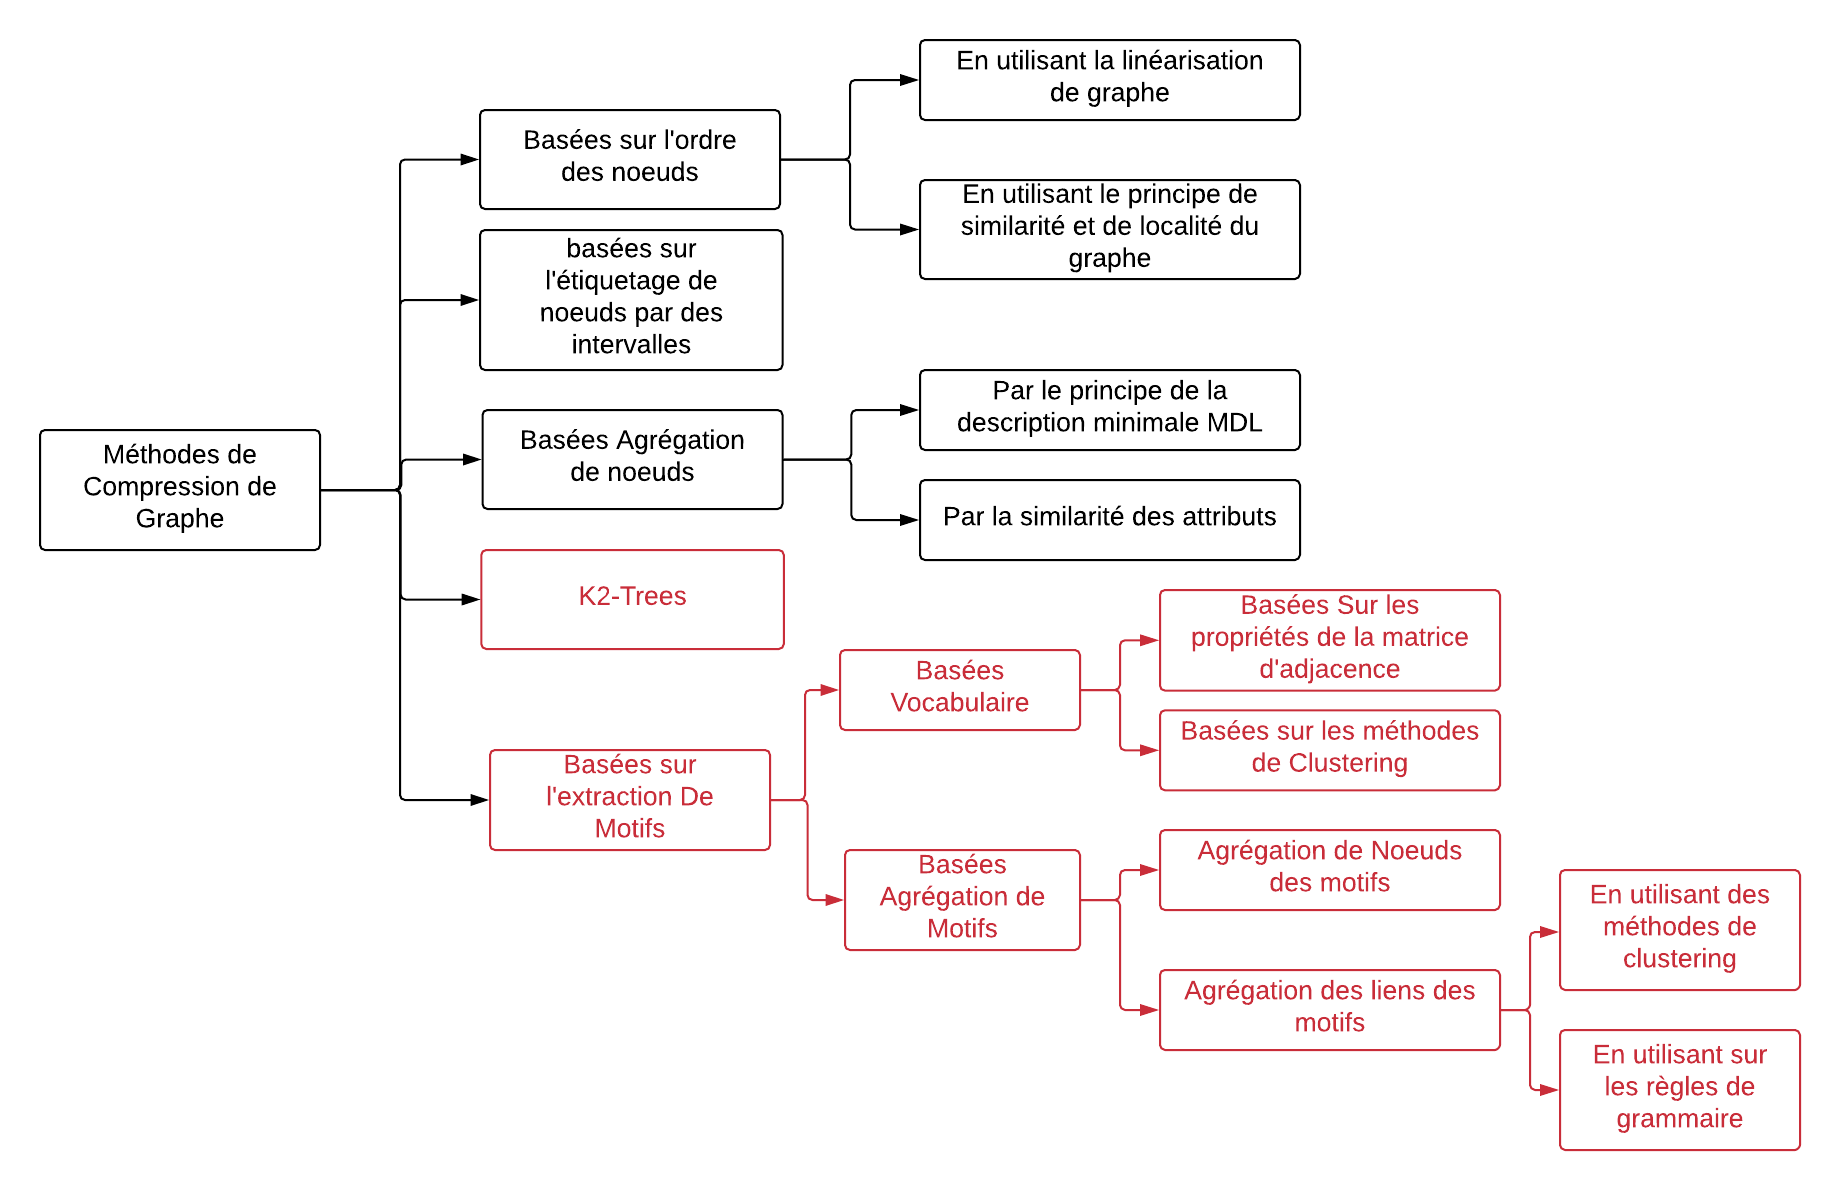
\includegraphics[scale=0.6]{./ressources/image/classif.png}
		\caption{Classification proposées des méthodes de compression}
	\end{figure}





